\documentclass[problem]{mcs}

\begin{pcomments}
    \pcomment{TP_a_bogus_tiling_induction}
    \pcomment{renamed from TP_A_Bogus_Induction}
    \pcomment{Written by EGM 01/30/13}
\end{pcomments}

\pkeywords{
induction
Tiles
Bill_Gates
bogus
logical_error
stategic_error
}

\begin{problem}
Frank Gehry has changed his mind.  Instead of the L-shaped tiles shown
in figure~\ref{fig:2Ltile}, he wants to use an odd offset pattern of
tiles (or its mirror-image reflection), as shown in
\ref{fig:offsettile}.  To prove this is possible, he uses reasoning
similar to the proof in~\ref{subsec:tile_induction}. However, unlike the
proof in the text, this proof is flawed.  Which part of the proof
below contains a logical error?

\begin{figure}

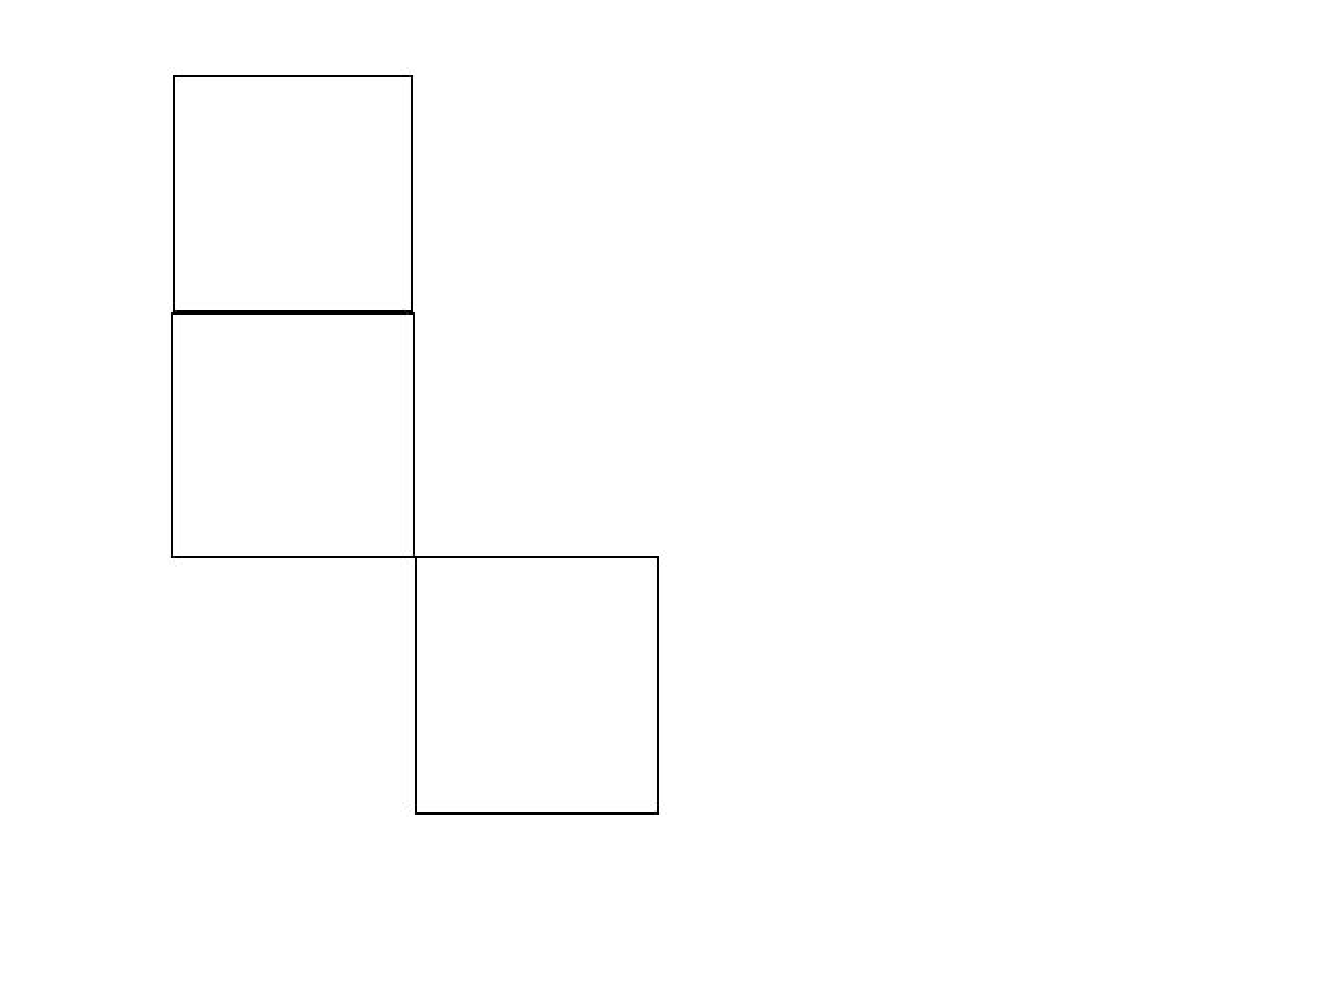
\includegraphics[height = 2in ]{Offset_tile}

\caption{Ghery's new tile.}
\label{fig:offsettile}
\end{figure}


\begin{falseclm*}\label{falsetiletheorem}
The proof is by induction.  Let $P(n)$ be the proposition that for
every location of Bill in a $2^n \times 2^n$ courtyard, there exists a
tiling of the remainder with the offset tile pattern.
\end{falseclm*}

\begin{falseproof}
\inductioncase{Base case}: $P(0)$ is true because Bill fills the
whole courtyard.

\inductioncase{Inductive step}: Assume that $P(n)$ is true for some
$n \geq 0$; that is, for every location of Bill in a $2^n \times 2^n$
courtyard, there exists a tiling of the remainder.  Divide the
$2^{n+1} \times 2^{n+1}$ courtyard into four quadrants, each $2^n
\times 2^n$.  One quadrant contains Bill (\textbf{B} in the diagram
below).  Place a temporary Bill (\textbf{X} in the diagram) in each of
the three squares lying near this quadrant as shown in
Figure~\ref{fig:bogustileimage}.

\begin{figure}

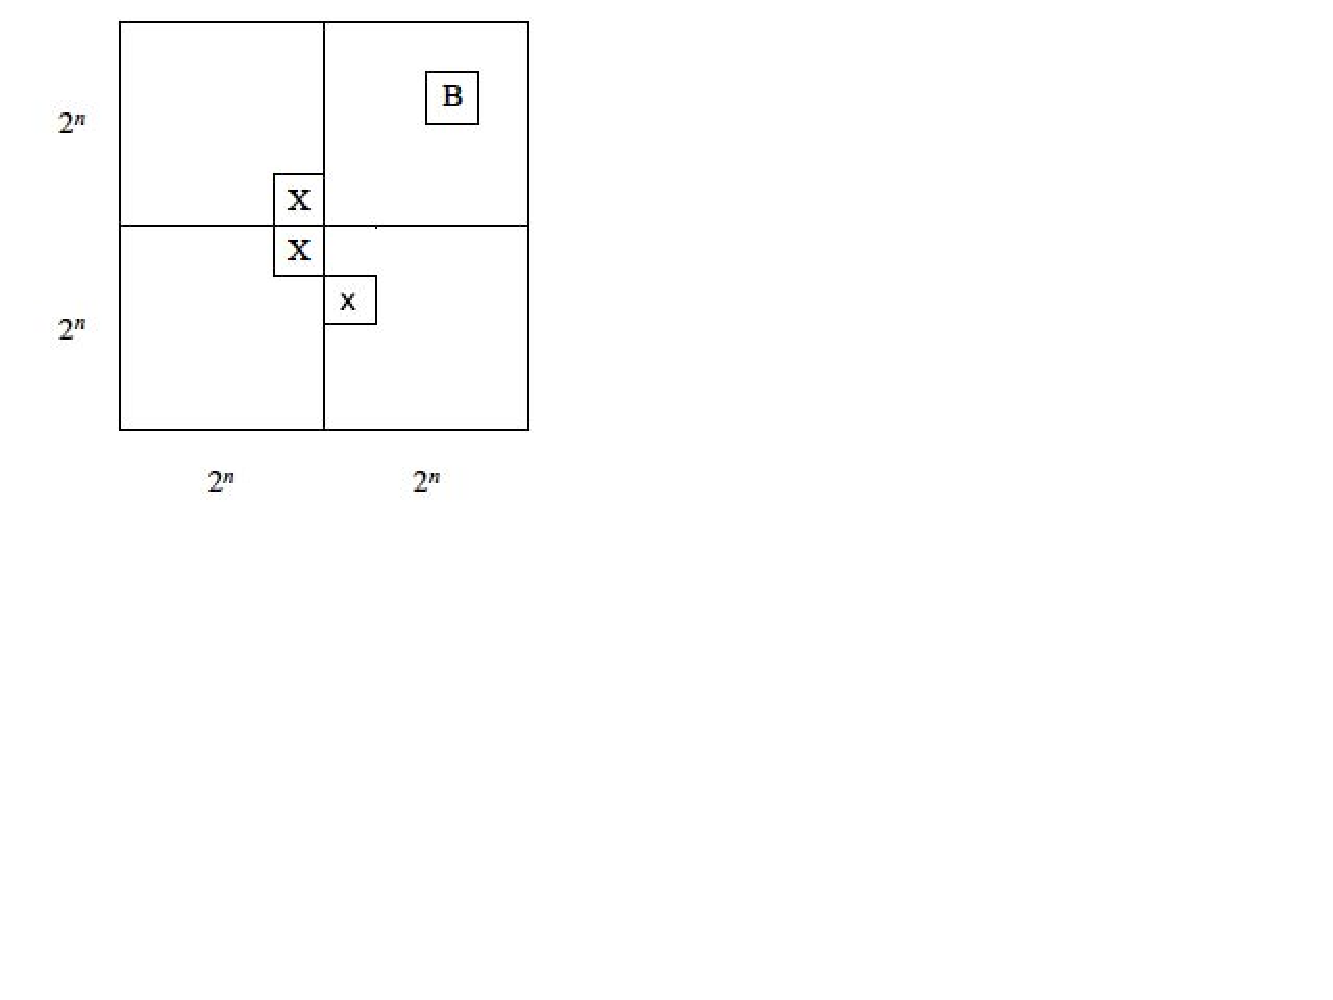
\includegraphics[trim = 0in 3in 5in 0in, clip, width = 3in]{Bogus_induction_step}

\caption{The induction hypothesis for the false theorem.}
\label{fig:bogustileimage}
\end{figure}

We can tile each of the four quadrants by the induction assumption.
Replacing the three temporary Bills with a single offset tile
completes the job.  This proves that $P(n)$ implies $P(n+1)$ for all
$n \geq 0$.  Thus $P(m)$ is true for all $m \in \naturals$, and the
ability to place Bill in the center of the courtyard follows as a
special case where we put Bill in a central square.
\end{falseproof}

%\hint Consider $n=1$.

\begin{solution}
The diagram in this problem is misleading.  It makes it appear that when
we assume the induction hypothesis, there will always be room for an
offset tile.  However, the diagram here is a shortcut.  Just like the
list $0, 1, 2\cdots n$ might only go up to $n=1$, the courtyards might
be significantly smaller than the one we've drawn.  Specifially, when
$n=1$, the $2 \times 2$ courtyard can fit exactly Bill and an L-shaped
tile, but cannot fit an offset tile at all.
\end{solution}

\end{problem}

\endinput
